\documentclass[letterpaper,12pt]{article}

\usepackage{fullpage} % Package to use full page
\usepackage{parskip} % Package to tweak paragraph skipping
\usepackage{tikz} % Package for drawing
\usepackage{mathtools}
\usepackage{hyperref}
\usepackage{amsfonts}
\usepackage{fancyhdr}
\usepackage{times}
\usepackage{changepage}
\usepackage{amssymb}
\usepackage{amsthm}
\usepackage{amsmath}
\usepackage[spanish]{babel}
\usepackage{graphicx}
\theoremstyle{plain}
\newtheorem{theorem}{Theorem}
\newcommand{\stirlingI}[2]{\genfrac{[}{]}{0pt}{}{#1}{#2}}
\newcommand{\stirlingII}[2]{\genfrac{{}{}}{0pt}{}{#1}{#2}}

\usepackage{authblk} % Paquete para manejar autores y afiliaciones
\renewcommand\Authand{ y } % Cambiar "and" por "y"

\title{Trabajo práctico 5: } % Título del documento

\author[1]{Ignacio Lembo Ferrari \thanks{Correo electrónico: ignacio.lembo@ib.edu.ar}}
\affil[1]{Instituto Balseiro}
%\affil[2]{Departamento de Física, Universidad de Ejemplo}

\date{\vspace{-4ex}}

\begin{document}

\maketitle

\section{Ejercicio 2 - Glucólisis}

La glucólisis es un proceso metabólico fundamental de los seres vivos, mediante el cual obtienen energía descomponiendo azúcar. Un modelo matemático de una de las reacciones involucradas es el siguiente:

\begin{align}
\dot{x}(t) &= -x + ay + x^2y \equiv f(x, y), \\
\dot{y}(t) &= \frac{1}{2} - ay - x^2y \equiv g(x, y),
\end{align}

donde $x(t)$ es la concentración de ADP, $y(t)$ es la de la glucosa-6-fosfato y $a \geq 0$ es un parámetro de la cinética química.
\begin{itemize}
    \item Muestre que hay un único equilibrio (encuéntrelo).
    \item Para $a = \frac{1}{2}$, grafique las nulclinas en el espacio de fases e identifique las regiones donde $f > 0$, $f < 0$, $g > 0$ y $g < 0$. En cada una de estas regiones, indique cualitativamente la dirección del flujo.
    \item Analice la estabilidad lineal del equilibrio.
    \item Considerando $a$ como un parámetro de control, muestre que existe una bifurcación. Dibuje cualitativamente el flujo en la proximidad del punto fijo para $a < a_c$ y $a > a_c$ ($a_c$ es el valor del parámetro de control donde se produce la bifurcación).
    \item Bonus: sabiendo que hay sólo un equilibrio y que las concentraciones no divergen al infinito, explique si existen ciclos de concentración (soluciones periódicas) para algún valor del parámetro $a$.
\end{itemize}


\subsection{Punto de equilibrio}

Para encontrar el equilibrio del sistema, necesitamos encontrar los puntos $(x^*, y^*)$ donde $\dot{x} = \dot{y} = 0$. Es decir, debemos resolver el sistema de ecuaciones:

\begin{equation}
    \begin{cases}
    0 &= -x + ay + x^2 y \\
    0 &= \frac{1}{2} - ay - x^2 y
    \end{cases}
\end{equation}

Resolviendo este sistema de ecuaciones llegamos a que el único punto de equilibrio es $(x^*, y^*) = \left(\frac{1}{2}, \frac{2}{4a +1}\right)$ donde $4a+1 \neq 0$. 

\subsection{Nulclinas y análisis de estabilidad}















\section{Descripción del problema}

Se tiene un conjunto de $q$ autos en una carretera que modelamos como una linea recta infinita, donde cada auto tiene una velocidad inicial dada por una cierta distribución de probabilidad y todos se mueven en la misma dirección. La regla es que los autos no se pueden pasar entre sí, es decir, si un auto en la posición $i$ alcanza al auto $i+1$ que está delante, se ve obligado a disminuir su velocidad para igualar la del auto $i+1$. De esta manera, se formarán trenes de autos. Las ideas principales de este trabajo son: dada una distribución de probabilidad de las velocidades iniciales de cada auto, encontrar la distribución del tamaño o longitud de trenes de autos formados y la distribución de probabilidad de la cantidad de trenes de autos. Para esto realizamos un desarrollo tanto teórico como computacional.


\section{Desarrollo teórico}

En primer lugar, de la descripción del problema podemos inferir las siguientes propiedades. Dado un tren de autos, en el estado estacionario se tiene que 
\begin{itemize}
    \item Una vez formado el tren de autos, el mismo no se puede desarmar. Solo se pueden añadir autos.
    \item Dado un auto con velocidad $v_i$ se formará un tren compuesto por todos los autos que están detrás de este con velocidad $v_j$ mayor o igual a $v_i$.
    \item Las velocidades de los autos que encabezan los trenes siguen una función decreciente con la posición.
    \item Todos los autos conservan la posición ya que no se pueden pasar entre sí.
\end{itemize}

Es importante destacar que una vez establecidas las velocidades iniciales, el problema es determinista, en el sentido que una vez que se conocen dichas velocidades se pueden determinar exactamente los trenes formados y su tamaño.

\subsection{Distribución de probabilidad del largo de trenes \label{sec:distlargo}}

En esta sección estudiaremos la distribución de probabilidad del largo de trenes. En primer lugar, dada la distribución de velocidades iniciales $f_v(v)$, nos interesa calcular la probabilidad $P(m)$ de tener un tren de $m$ autos. Esto se puede pensar como: dado un auto que encabeza un tren con velocidad $v_T$, la probabilidad de tener $m-1$ autos con velocidad $v>v_T$ se escribe, en el caso de que $m < q$, como 
\begin{equation}
    P(m|v_T) = P(v>v_T)^{m-1} P(v<v_T),
\end{equation}
y si $m=q$,
\begin{equation}
    P(m=q|v_T) = P(v>v_T)^{m}.
\end{equation}

Esto da la probabilidad de tener un tren de $m$ autos dado que la velocidad del primer auto del tren es $v_T$. Luego, la probabilidad de tener un auto con velocidad $v_T$ está dada por $f_v(v_T)$. Para $m<q$ la probabilidad de tener un tren de $m$ autos es 
\begin{align}
    P(m) &= \int_0^{\infty} \text{d}v_T ~ P(m|v_T) f_v(v_T) = \\
    &=\int_0^{\infty} \text{d}v_T ~ P(v>v_T)^{m-1} P(v<v_T) f_v(v_T) = \\    
    &=  \int_0^{\infty} \text{d} v_T ~ \biggr[ \int_{v_T}^{\infty}\text{d}v ~f_v(v)  \biggr]^{m-1} \int_0^{v_T} \text{d}v ~f_v(v).
    \label{pk}
\end{align}
Esto puede simplificarse aún más realizando un cambio de variables y utilizando que
\begin{equation}
    f_v(v_T)=-\frac{\text{d}}{\text{d}v_T}\left(\int_{v_T}^{\infty}\text{d}v ~f_v(v)\right)=-\frac{\text{d}a}{\text{d}v_T}\text{.}
\end{equation}

Teniendo en cuenta que cuando $v_T \to 0$, $a \to 1$ y $v_T \to \infty$, $a \to 0$, la Ec. (\ref{pk}) se convierte en
\begin{equation}
    P(m)=\int_0^1 \text{d}a\left(a^{m-1}-a^{m}\right)=\frac{1}{m(m+1)}\text{.}
    \label{kk1}
\end{equation}

De manera similar, se puede realizar el cálculo cuando el tren es de largo $q$
\begin{align}
    P(m=q) &= \int_0^{\infty} \text{d}v_T ~ P(m|v_T) f_v(v_T) = \\    
    &=  \int_0^{\infty} \text{d} v_T ~ \biggr[ \int_{v_T}^{\infty}\text{d}v ~f_v(v)  \biggr]^{q}\text{,}
\end{align}
obteniendo finalmente
\begin{equation}
    P(m=q)= \frac{1}{q}.
    \label{ec:m=q}
\end{equation}

Es notable como las Ecs. (\ref{kk1}) y (\ref{ec:m=q}) son válidas para cualquier cantidad de autos $q$. Más aún, la distribución de probabilidad del largo de un tren no depende de la distribución inicial de velocidades $f_v(v)$. 

La Ec. (\ref{kk1}) da la probabilidad de tener un tren formado por $m<q$ autos dado que el primero del tren tiene velocidad $v_T$, luego podemos calcular la probabilidad de tener un segundo tren detrás del primer tren con $m_2$ autos. La probabilidad en este caso va a venir dada por una ecuación similar a la anterior pero teniendo en cuenta que ahora el primer tren tiene velocidad $v_1$ y $m_1$ autos y se satisface que $v_1 > v_2$ y $m_1 + m_2 < q$
\begin{equation}
    P_2(m_2) = \int_0^{\infty} \text{d}v_1 f_v(v_1) \int_0^{v_1} \text{d}v_2 ~ P(m_2|v_2) f_v(v_2).
\end{equation}
Mediante un desarrollo similar al realizado para el primer tren se obtiene
\begin{equation}
    P_2(m_2) = \int_0^{\infty} \text{d}v_1 f_v(v_1) \left(\frac{1-a^{m_2}}{m_2}\right)\text{.}
\end{equation}

En los casos de más trenes, se obtiene de la misma manera una concatenación de integrales, de las cuales no se puede obtener una solución analítica.

\subsection{Distribución de probabilidad de la cantidad de trenes}

Ahora estudiaremos la distribución de probabilidad de la cantidad de trenes de autos formados para $q$ autos en total. Pensemos inicialmente en un caso discreto donde tenemos con $n$ velocidades que se pueden repetir entre los autos. Es fácil ver, que hay $n^q$ formas de distribuir las $n$ velocidades en $q$ autos. El número de formas de construir un tren con velocidad de grupo $v$ y $m$ miembros es 
\begin{equation}
    G(v,m) = (n - v + 1)^{m-1}.
\end{equation}
Esto es porque, estamos contando todas las formas de tener $m-1$ autos (no contamos el primer auto con velocidad $v$) con velocidad mayor que el primer auto. Luego, el número de formas de tener un solo tren de autos es
\begin{equation}
    N_1 (n,q) = \sum_{1 \leq v_1 \leq n} (n - v_1 + 1)^{q-1} = \sum_{1\leq k\leq n} k^{q-1},
\end{equation}
donde $k = n - v_1 + 1$ y sumamos sobre todas las posibles velocidades que puede tomar el auto que encabeza el tren.

Para dos trenes de autos, tal que se cumple que $m_1 + m_2 = q$, donde mientras se cumpla $1 \leq v_2 \leq v_1 \leq n$ tenemos $G_1(v_1,m_1)$ y $G_2(v_2,m_2)$ formas de construir cada tren. Entonces, la cantidad de formas totales de distribuir las velocidades será $(n - v_1 + 1)^{m_1-1}(n - v_2 + 1)^{m_2-1}$, es decir, cantidad de formas de armar el primer tren multiplicado por la cantidad de formas de armar el segundo tren sujeto a $v_1 > v_2$. Luego, 
\begin{equation}
N_2 (n,q) = \sum_{\substack{m_1 + m_2 = q \\ m_i \geq 1}} \sum_{1 \leq v_2 \leq v_1 \leq n} (n - v_1 + 1)^{m_1-1} (n - v_2 + 1)^{m_2-1}, 
\end{equation}
donde $k_i = n - v_i + 1$ con $i = 1,2$. 

La probabilidad de tener 2 trenes es el número de configuraciones $N_2(g)$ sobre el número total de configuraciones $n^q$
\begin{align}
P_2(q) = \frac{N_2}{n^q} &= \frac{1}{n^q} \sum_{\substack{m_1 + m_2 = q \\ m_i \geq 1}} \sum_{1 \leq k_1 < k_2 \leq n} k_1^{m_1-1} k_2^{m_2-1}\\
&=\frac{1}{n^2} \sum_{\substack{m_1 + m_2 = q \\ m_i \geq 1}} \sum_{1 \leq k_1 < k_2 \leq n} \biggr(\frac{k_1}{n}\biggr)^{m_1-1} \biggr(\frac{k_2}{n}\biggr)^{m_2-1}.
\end{align}

Esto se puede generalizar para una configuración de $q$ autos, $g$ trenes de autos y $m_i$ cantidad de autos por tren con $i$ entre 1 y $g$ 
\begin{equation}
    P_g(q) = \frac{1}{n^g} \sum_{\substack{m_1+...+m_g = q \\  m_i \geq 1}}  \sum_{1 \leq k_1 < ...< k_g \leq n} k_1^{m_1-1} ... k_g^{m_g-1}. 
\end{equation}

Ahora pasamos al continuo $n \to \infty$ y, definiendo $k_j/n = x_j$ y absorbiendo el término $\frac{1}{n^g}$ en el cambio de variables $d\vec{x} = dx_1 .. dx_g = \frac{d\vec{k}}{n^g}$ tenemos que la probabilidad de tener $g$ trenes de autos para $q$ autos en total es 

\begin{align}
P_g (q) &= \sum_{m_1+...+m_g = q} \int_{0 \leq x_1 < ... < x_g  \leq 1} \prod_{1 \leq j \leq g} (x_j^{m_j-1}) d\vec{x} \\
&= \sum_{m_1+...+m_g = q} \int_{x_3<...<x_g\leq 1} \int_{x_1}^{x_3} \underbrace{\int_0^{x_2} dx_1 x_1^{m_1-1}}_{\frac{x^{m_1}}{m_1}|_0^{x_2}  = \frac{x_2^{m_1}}{m_1}} dx_2 x_2^{m_2-1} \prod_{3 \leq j \leq g} x_j^{m_j-1} dx_j = \\
&= \sum_{m_1+...+m_g = q} \frac{1}{m_1}  \int_{x_4<...<x_g\leq 1} \underbrace{\int_{x_1}^{x_3} x_2^{m_1+m_2-1}  dx_2}_{\frac{1}{m_1+m_2} x_2^{m_1+m_2} |_0^{x_3} = \frac{1}{m_1+m_2} x_3^{m_1+m_2} } dx_3 x_3^{m_3-1} \prod_{3 \leq j \leq g} x_j^{m_j-1} dx_j  \\
&= \sum_{\substack{m_1+...+m_g = q \\ m_i \geq 1}} \frac{1}{m_1} \frac{1}{m_1+m_2} ... \frac{1}{m_1+ ... + m_g}.
\end{align} 

Veamos en el resultado anterior que $m_1 + ... + m_g = q$ son todas las posibles formas de sumar $q$ con $g$ números naturales y además el término $1/(m_1+ ... + m_g)$ puede factorizarse de la expresión ya que $q$ es constante obteniendo 
\begin{equation}
P_g (q) = \frac{1}{q} \sum_{\substack{m_1+...+m_g = q \\ m_i \geq 1}} \frac{1}{m_1} \frac{1}{m_1+m_2} ... \frac{1}{m_1+ ... + m_{g-1}}
\label{ec:casiPg}
\end{equation}
Por otro lado, dado que $m_g$ toma todos los valores entre 1 y $q - (g-1)$, ya que $m_j \geq 1$, los valores de $m_j$ con $j = 1,..,g-1$ que quedan en los cocientes de la Ec. (\ref{ec:casiPg}) son todas las posibles formas de sumar los números entre $(g-1)$ y $q-1$ con $g-1$ números naturales. Luego, teniendo en cuenta esto y el resultado obtenido para $P_g(q)$ podemos reescribir la expresión como
\begin{equation}
P_g (q) = \frac{1}{q} \sum_{0 \leq g-1 \leq k \leq q-1 } P_{g-1}(k).
\label{ec:recursion}
\end{equation}
Donde obtuvimos una fórmula de recurrencia para la probabilidad y como condiciones iniciales para la fórmula de recurrencia podemos tomar como condición inicial que 0 autos solo pueden estar en un tren vacío o que un tren vacío solo puede tener 0 autos, es decir 
\begin{equation}
P_g(0) = \delta_{g,0}, \hspace{1cm} P_0(q) = \delta_{q,0}.
\end{equation}

Consideremos ahora la siguiente identidad para los números de Stirling de primer orden 
\begin{equation}
    \stirlingI{q+1}{g+1} = \sum_{k=g}^{q} \stirlingI{k}{g} \frac{q!}{k!},
\end{equation}
donde $g$ es el número trenes de autos y $q$ el número total de autos, realizando un cambio de variables podemos llevar la identidad a la siguiente expresión 
\begin{align}
    \stirlingI{q}{g} &= \frac{1}{q} \sum_{k=g-1}^{q-1} \stirlingI{k}{g-1} \frac{(q-1)!}{k!} \\
    \biggr( \frac{1}{q!} \stirlingI{q}{g} \biggr) &= \frac{1}{q} \sum_{k=g-1}^{q-1} \biggr(  \frac{1}{k!} \stirlingI{k}{g-1} \biggr)
    \label{ec:stirling}
\end{align}
En particular, podemos ver que la relación a la que llegamos en términos del número de Stirling satisface la misma relación de recurrencia que la Ec. (\ref{ec:recursion}). Luego, para las mismas condiciones iniciales mencionadas podemos escribir la distribución de probabilidad para la cantidad de trenes de autos $g$, para una cantidad total de autos $q$ como
\begin{equation}
    P_g(q) = \frac{1}{q!} \stirlingI{q}{g}.
    \label{ec:distfinal}
\end{equation}
Se ha demostrado \cite{benjamin_stirling_2002} que el valor medio de una distribución de probabilidad dada por la Ec. \ref{ec:distfinal} es el número armónico q-ésimo $H_q$
\begin{equation}
    \Bar{g}(q) = \sum_{g \leq q} \frac{g}{q!} \stirlingI{g}{q} = H_q,
    \label{ec:valormedio}
\end{equation}
donde 
\begin{equation}
    H_q = \sum_{k=1}^q \frac{1}{k}.
\end{equation}
Por lo tanto, el valor medio de la cantidad de trenes de autos $g$, cuya distribución de probabilidad está dada por Ec. (\ref{ec:distfinal}), es $H_q$. Estos resultados analíticos se contrastan en la sección \ref{sec:estacionario} con simulaciones realizadas para un conjunto de $q$ autos con velocidades iniciales dadas por una distribución de probabilidad log-normal obteniendo resultados satisfactorios.

\section{Implementación computacional}

Realizamos simulaciones computacionales para el problema planteado, tanto en el régimen transitorio como en el estacionario.

\subsection{Evolución del régimen transitorio}

Para observar el transitorio utilizamos una única realización con $q=1000$ autos inicialmente equiespaciados a una distancia $d=10$. Se les asignó a cada auto estocásticamente una velocidad según una distribución de probabilidad log-normal dada por
\begin{equation}
f_v (v)= \frac{1}{v\sigma \sqrt{2\pi}} \exp\left(-\frac{(\ln v - \mu)^2}{2\sigma^2}\right),
\end{equation}
donde utilizamos $\mu=5/2$ y dos valores de $\sigma= 5/8$ y $1/10$. La Fig. \ref{fig:trans} muestra las gráficas en función del tiempo para estos datos donde se muestra la evolución de la cantidad de trenes (contando autos individuales como un tren) y la velocidad media de los mismos. Además, se puede observar cómo el tiempo de llegada al estacionario depende del parámetro $\sigma$. Esto se debe a que al disminuir dicho parámetro, las velocidades de los autos son más cercanas entre ellas y los autos necesitan más tiempo para alcanzarse entre sí.

\begin{figure}[h]
    \centering
    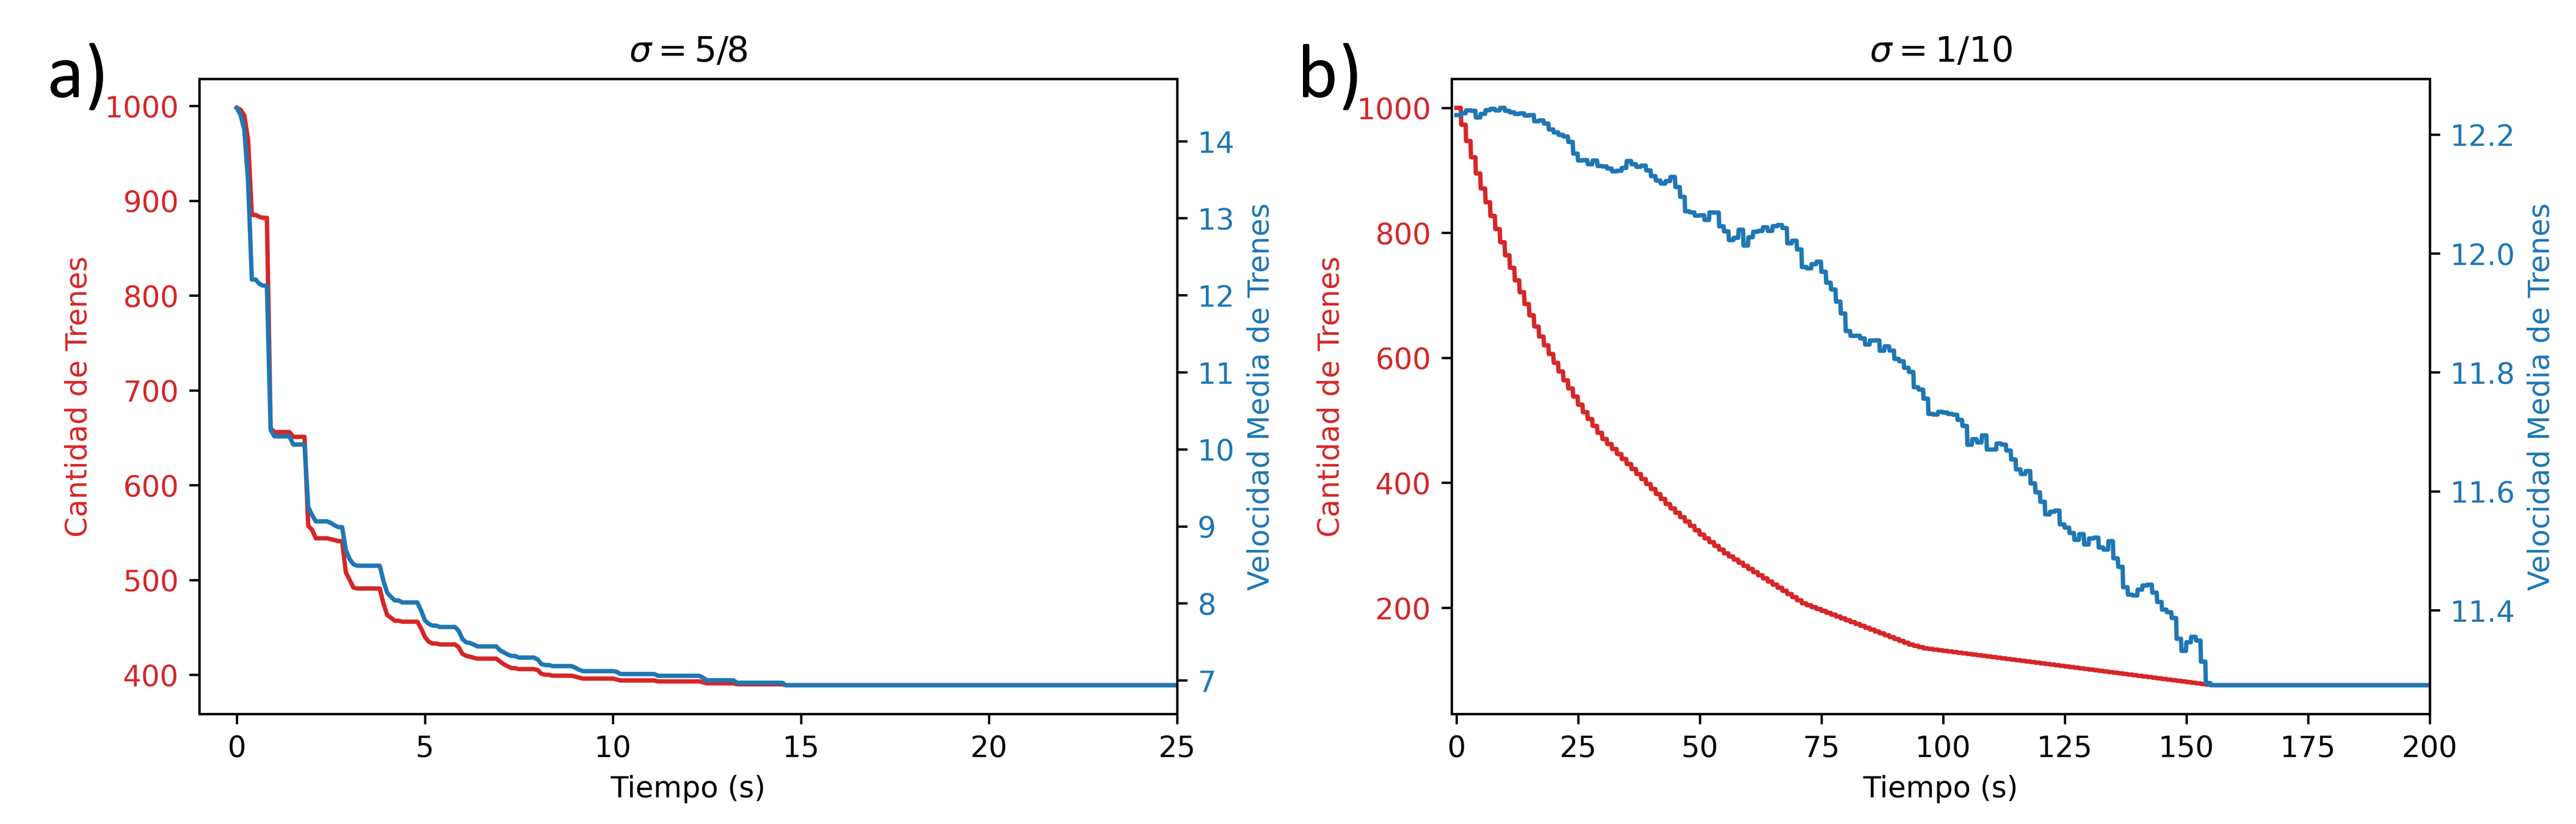
\includegraphics[width=\textwidth]{Transssss.png}
    \caption{Gráficas de cantidad de trenes y velocidad media de los mismos en función del tiempo. En rojo se muestra la evolución de la cantidad de trenes y en azul la velocidad media de los mismos. (a) Gráfica para $\sigma= 5/8$. (b) Gráfica para $\sigma= 1/10$}. 
    \label{fig:trans}
\end{figure}

\newpage

\subsection{Análisis del régimen estacionario \label{sec:estacionario}}

Realizamos simulaciones para el sistema en el estado estacionario, es decir cuando ya no se forman más trenes de autos. Utilizamos $q=1000$ autos y 100000 realizaciones del experimento para todos los casos que se presentan a continuación. 

En la Fig. \ref{fig:kprimer} se presenta la distribución de tamaños del primer tren para cada una de las realizaciones del experimento. Observamos como el cálculo analítico dado por la Ec. (\ref{kk1}) para $m<q$ se corresponde con el resultado obtenido mediante las simulaciones.

\begin{figure}[h]
    \centering
    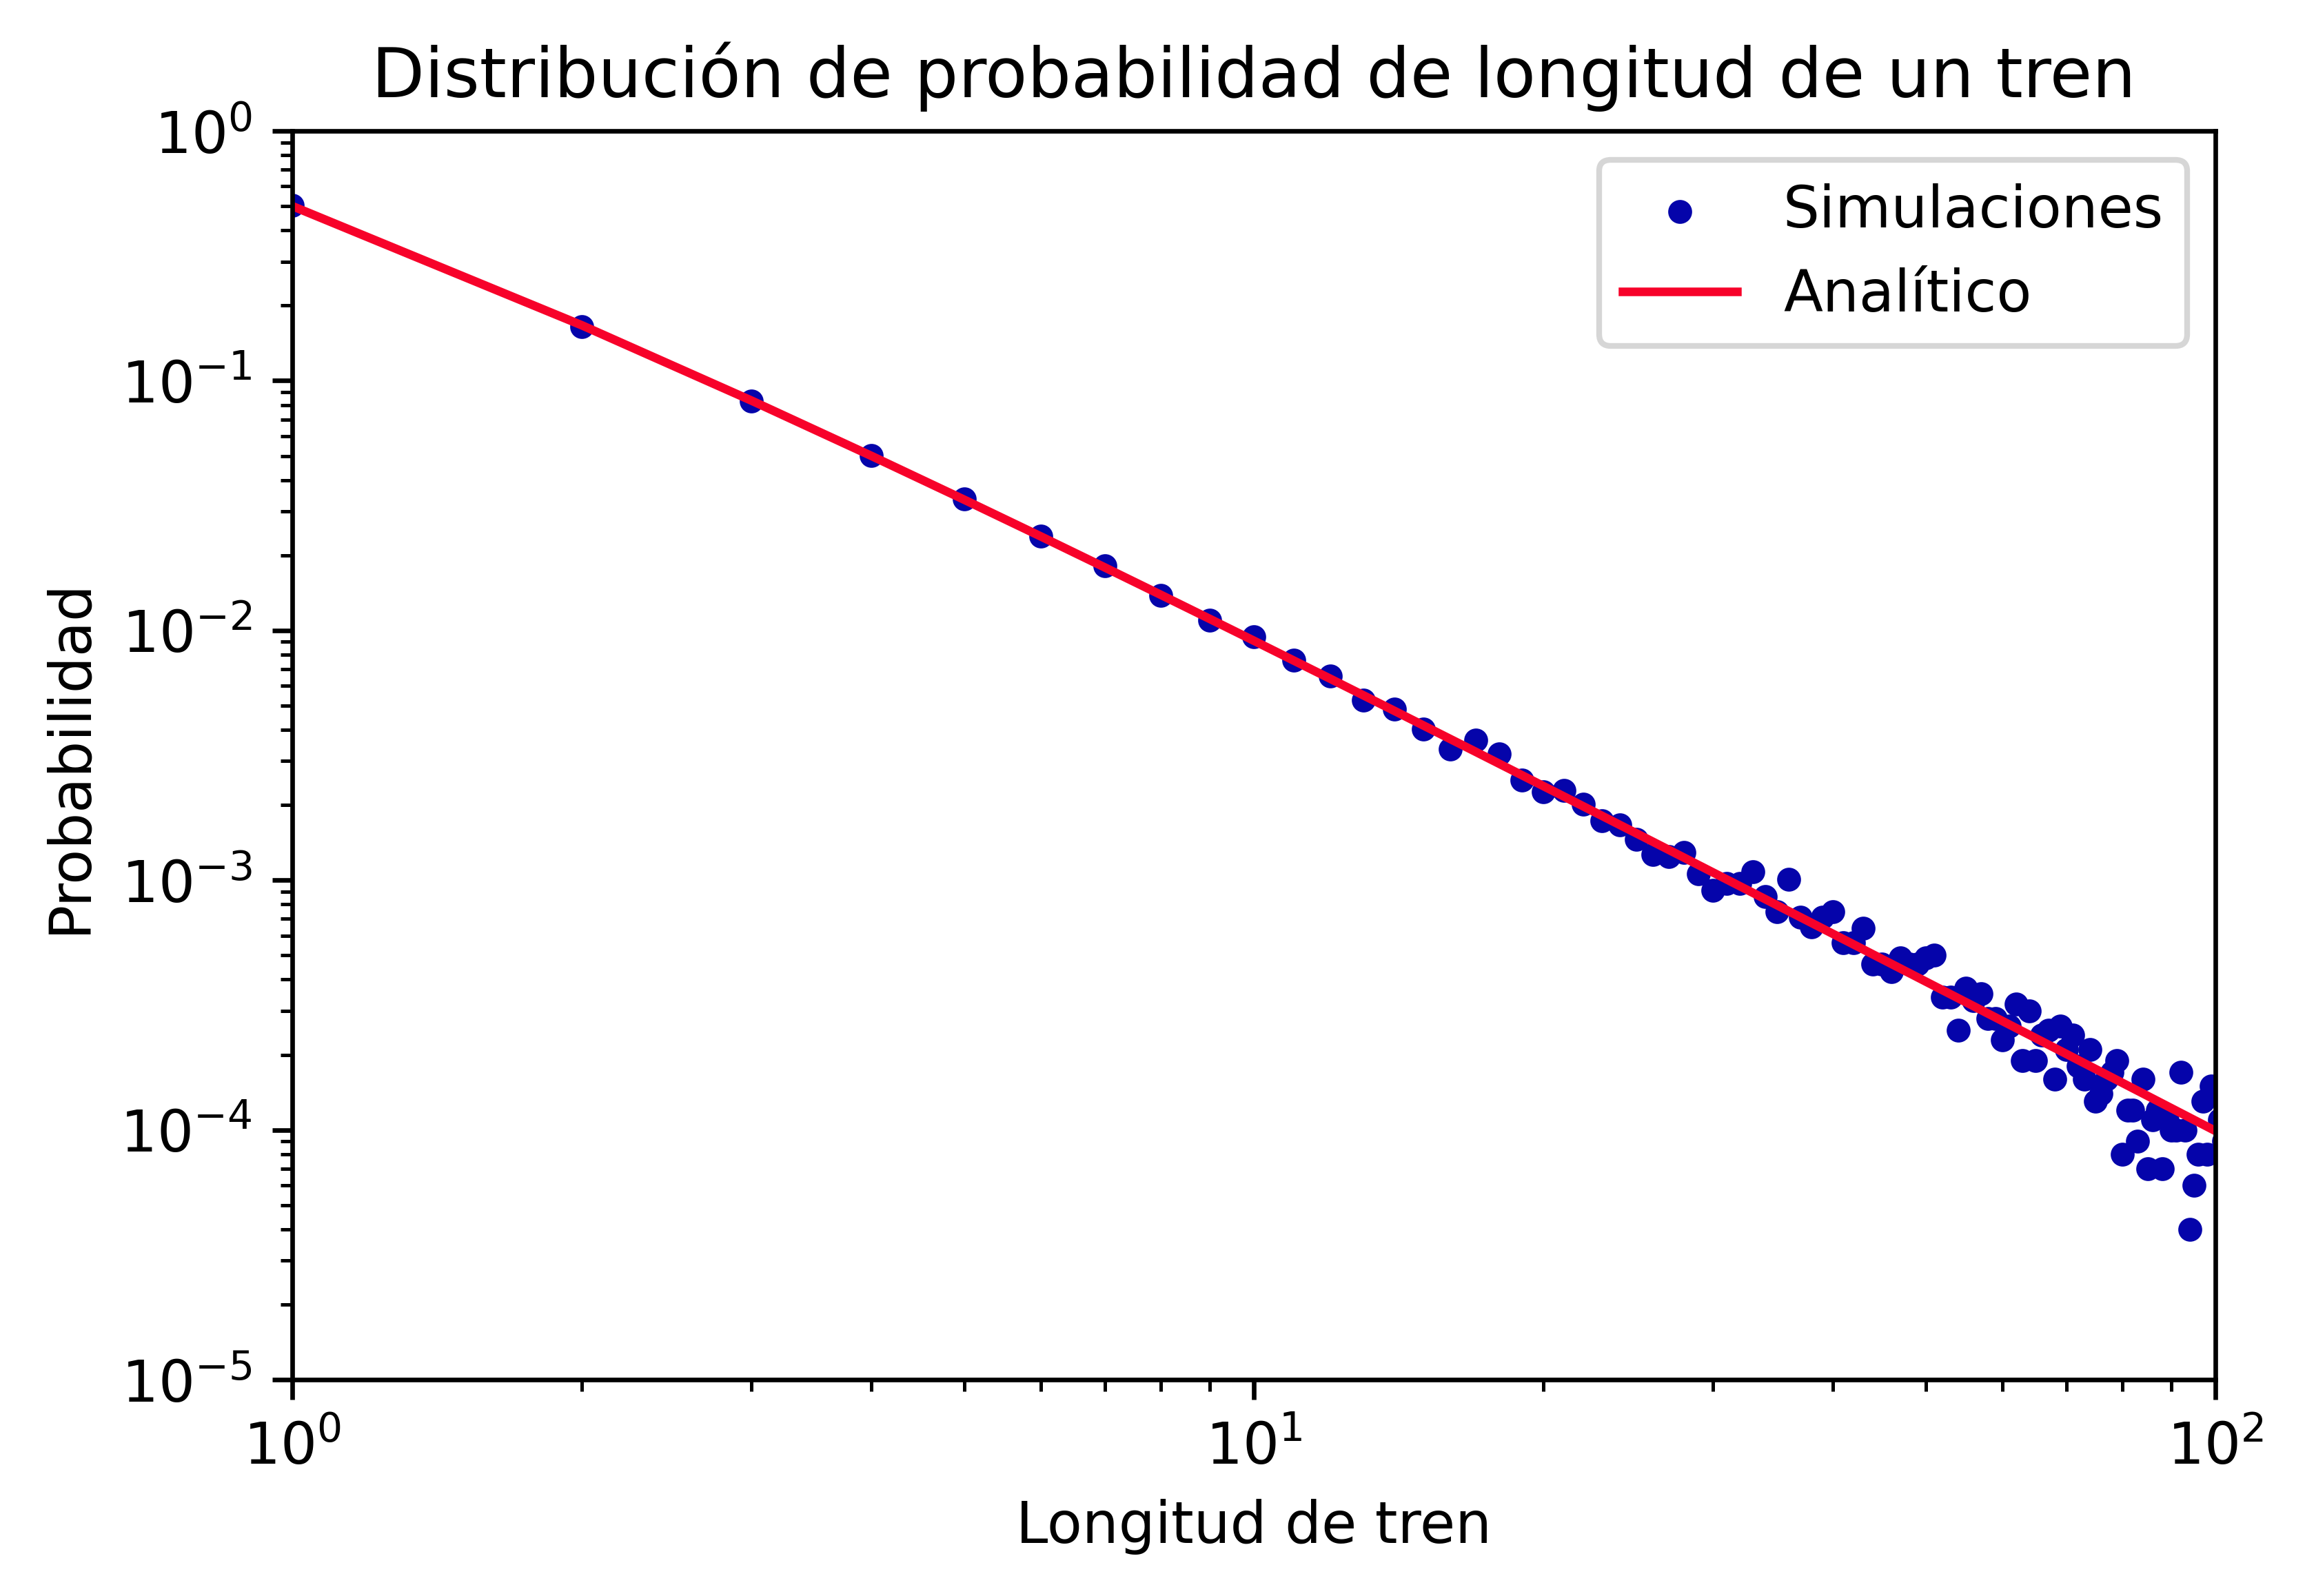
\includegraphics[width=0.5\textwidth]{kprimer.png}
    \caption{Gráfica en log-log de la distribución del largo del primer tren para una simulación con $q=1000$ autos y 100000 realizaciones del experimento. La curva roja es la distribución probabilidad de tamaño de un tren dada por $1/m(m+1)$. Vemos que la curva es altamente compatible con las simulaciones.}
    \label{fig:kprimer}
\end{figure}

\newpage 

Por otra parte, realizamos simulaciones donde tomamos la longitud de todos los trenes formados en cada realización, obteniendo de esta manera la distribución de probabilidad del tamaño de todos los trenes formados. 
Los resultados se presentan en la Fig. \ref{fig:ktodos}. En la sección \ref{sec:distlargo} mostramos que la distribución de probabilidad para dos o más trenes de autos formados tiene una expresión analítica compleja, no obstante en la Fig. \ref{fig:ktodos} podemos ver como esta distribución parece seguir una ley de potencias de la forma $1/x$. Más aún, observamos que, para valores de longitud de tren grande, la distribución de probabilidad aumenta. Este fenómeno no es un error computacional, sino el efecto descripto anteriormente en la sección  \ref{sec:distlargo}, donde vimos que un tren de tamaño $q$ es más probable que uno de largo $q-1$.

\begin{figure}[h]
    \centering
    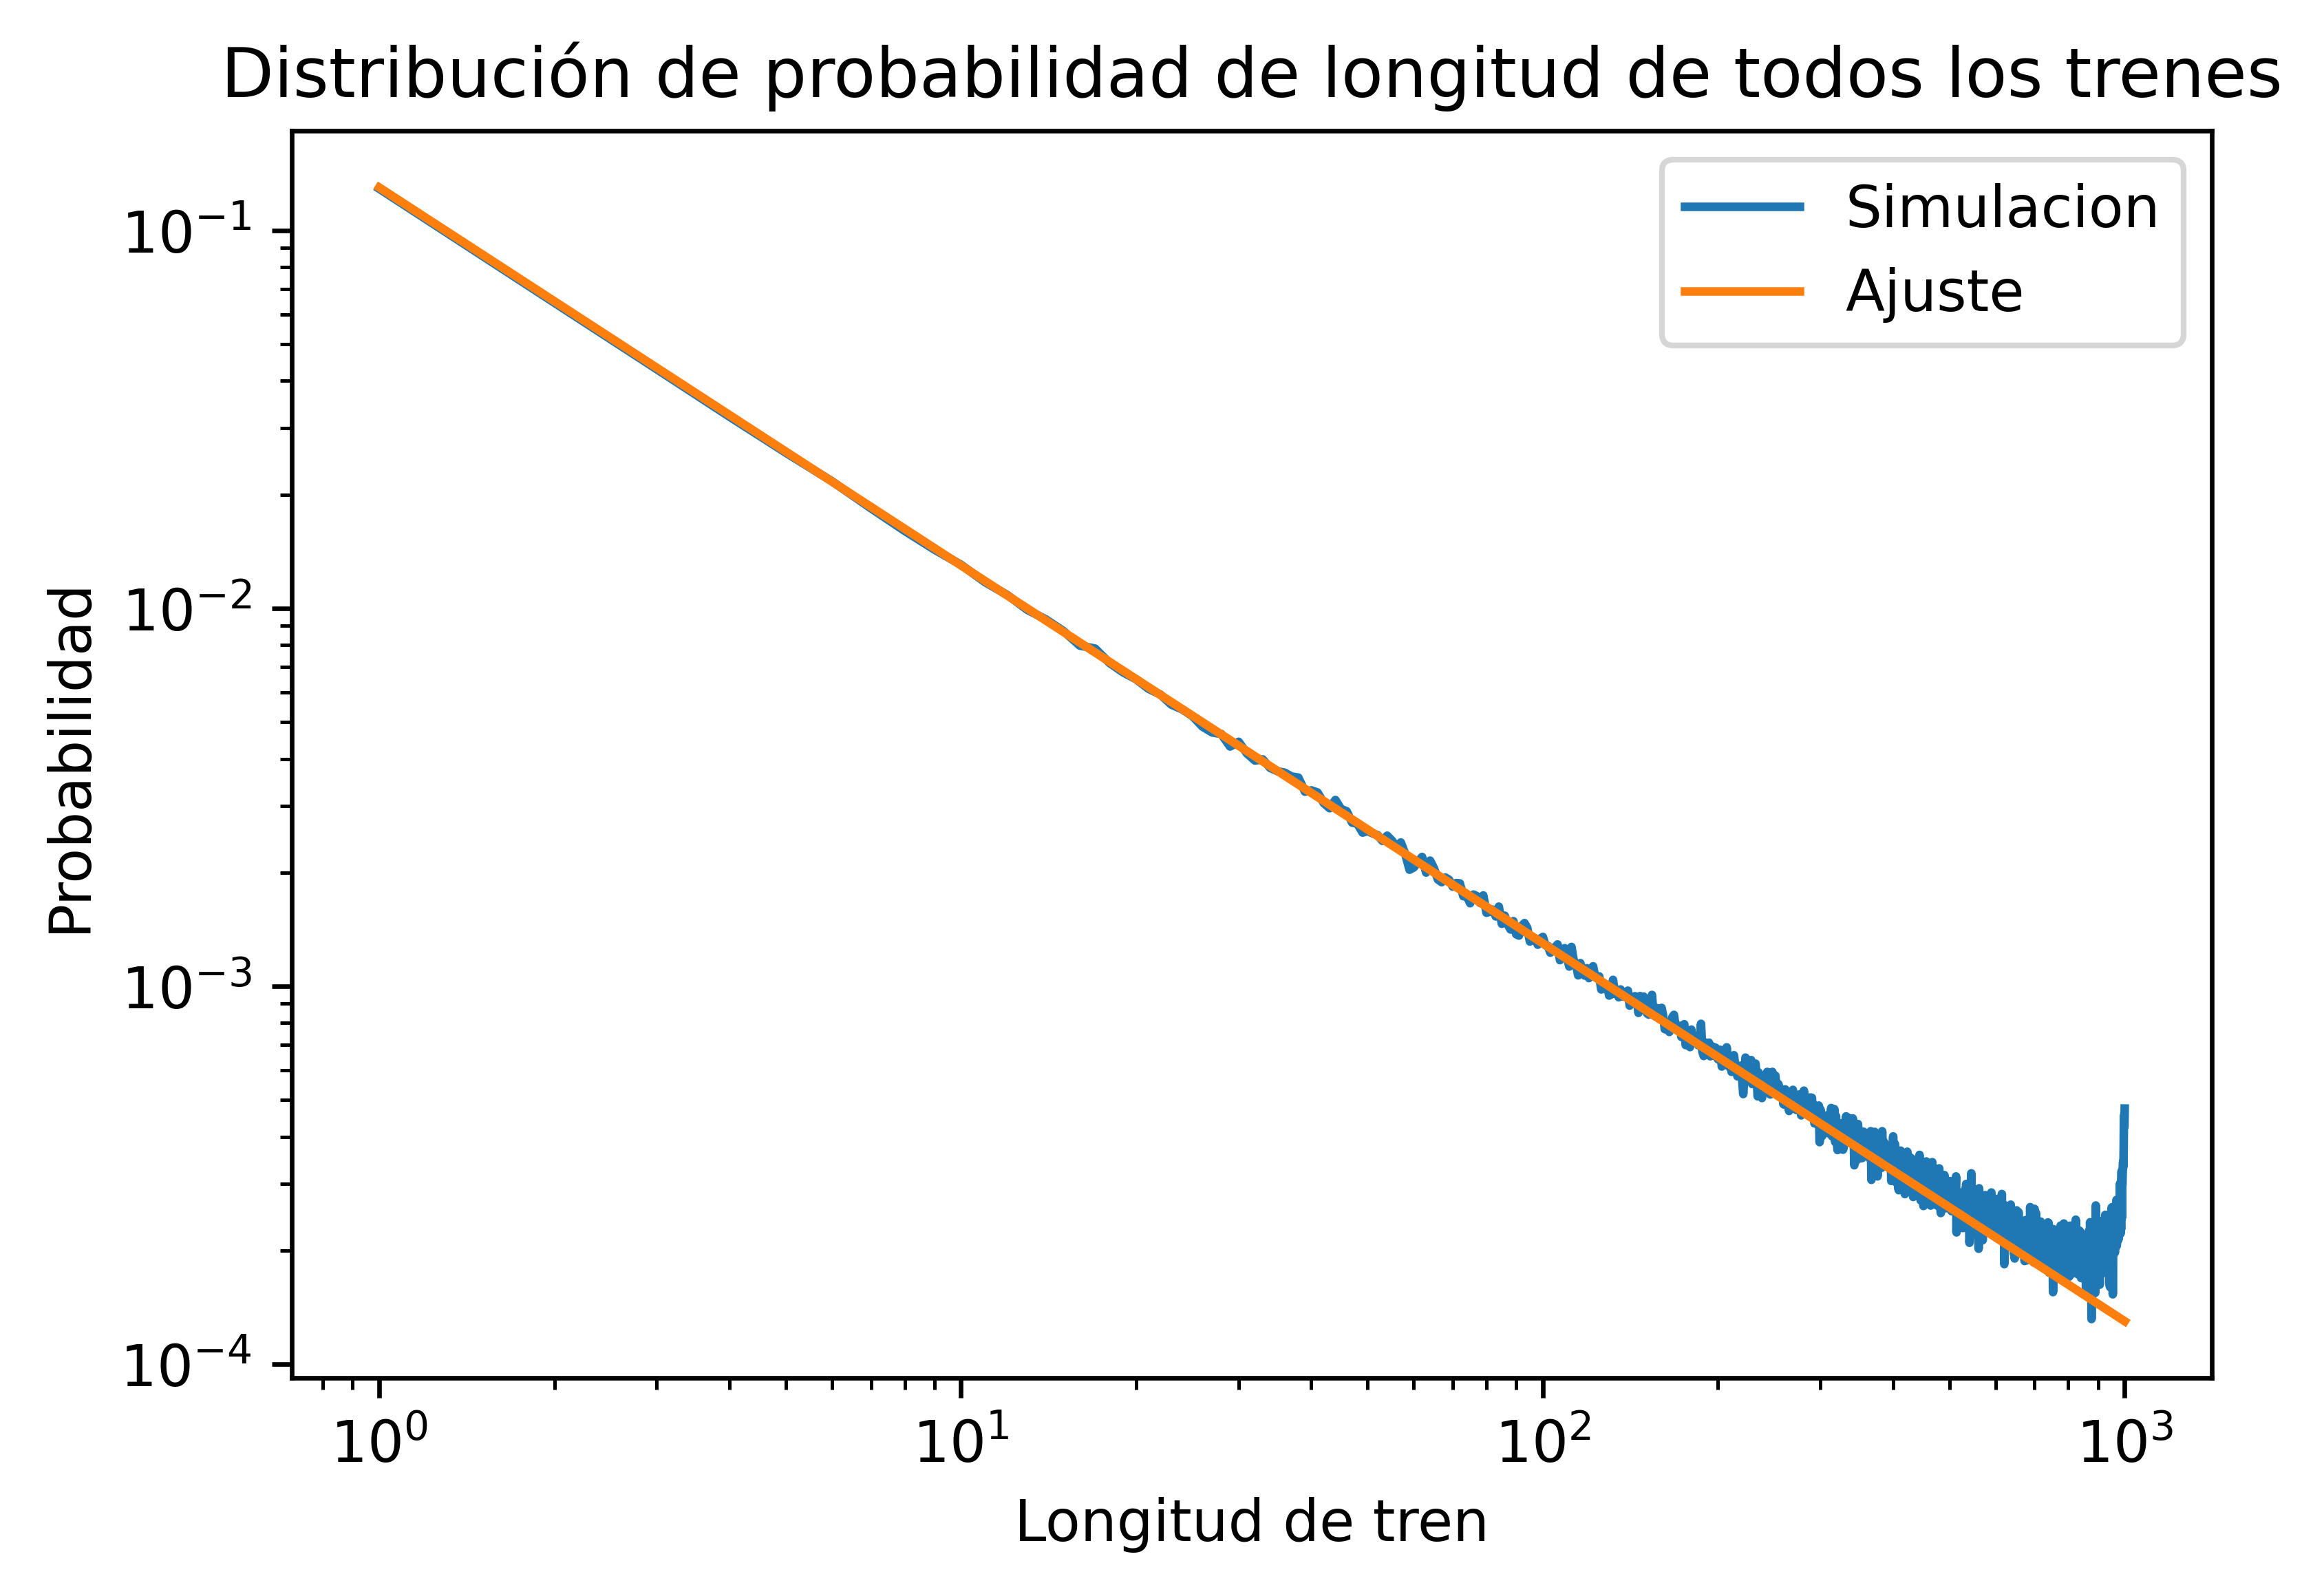
\includegraphics[width=0.5\textwidth]{ktodostrenes.png}
    \caption{Gráfica en log-log de la distribución del largo de todos los trenes para una simulación con $q=1000$ autos y 100000 realizaciones del experimento. Se ajustó una ley de potencias obteniendo un exponente de -1}
    \label{fig:ktodos}
\end{figure}


Finalmente, obtuvimos la distribución de probabilidad de la cantidad de trenes de autos formas, como muestra la Fig. \ref{fig:ntrenes}. Aquí observamos como las Ecs. (\ref{ec:distfinal}) y (\ref{ec:valormedio}) predicen correctamente la distribución y la media obtenidas mediante las simulaciones.

\begin{figure}[h]
    \centering
    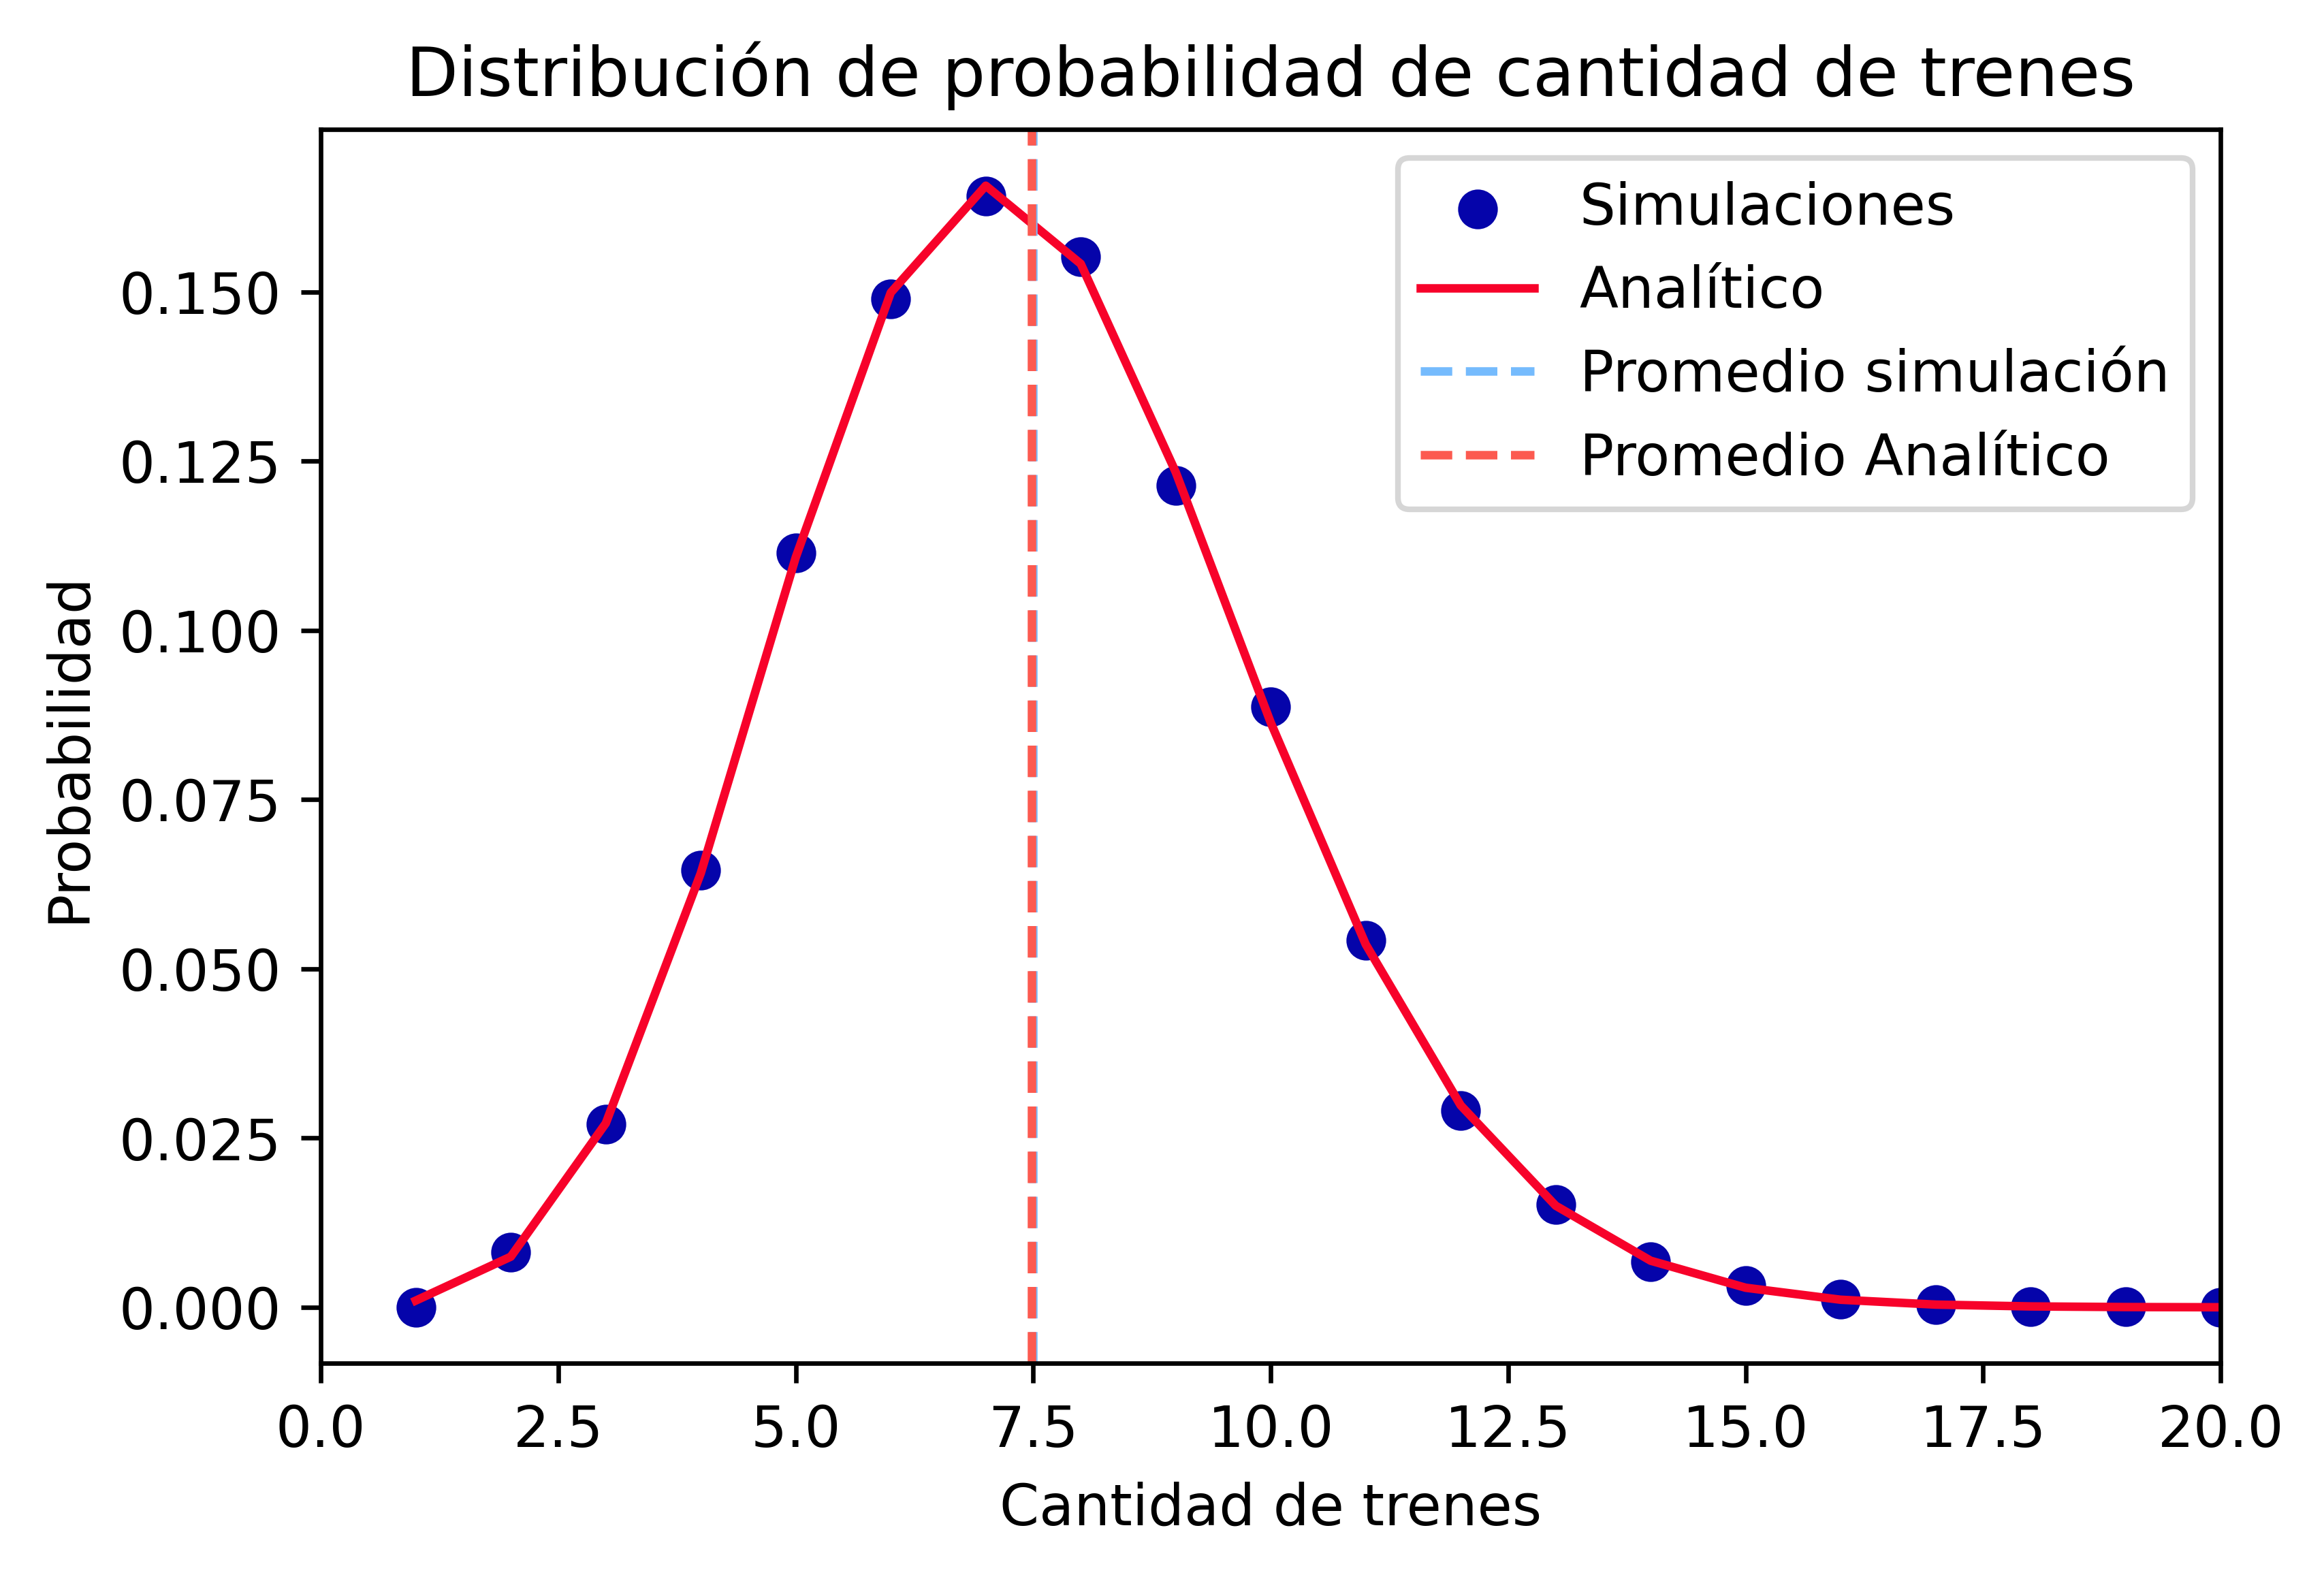
\includegraphics[width=0.6\textwidth]{ntrenes.png}
    \caption{Distribución de probabilidad de la cantidad de trenes en una realización. Los puntos muestran lo obtenido en la simulación y la linea continua roja el resultado analítico dado por la Ec. (\ref{ec:distfinal}). En linea discontinua se muestran los valores medios obtenidos analíticamente (dado por la Ec. (\ref{ec:valormedio})) y obtenido a partir de la simulación.}
    \label{fig:ntrenes}
\end{figure}

\section{Conclusiones}

A través del desarrollo teórico, se establecieron propiedades fundamentales de la dinámica de los trenes, y se derivaron expresiones analíticas para la distribución de tamaños de los trenes. Sea $q$ el número total de autos y $m$ el tamaño del tren de autos, se demostró que la distribución de probabilidades de tener un tren de tamaño $m<q$ sigue una ley $\frac{1}{m(m+1)}$ y, para $m=q$ una distribución de probabilidad dada por $\frac{1}{q}$. Además se encontró una relación de recurrencia que describe la distribución completa de la cantidad de trenes.

La implementación computacional permitió validar los resultados teóricos a través de simulaciones. Se observó la evolución temporal del sistema desde un estado inicial hasta el estacionario, evidenciando la dependencia del tiempo de convergencia con el parámetro de dispersión $\sigma$ de la distribución log-normal. Además, se compararon las distribuciones de tamaño de trenes obtenidas analíticamente con aquellas derivadas de simulaciones, encontrando una excelente concordancia.

En el régimen estacionario, se analizó la distribución de tamaños de los trenes, comportándose como una ley de potencias $1/m$. Se destacó la presencia de un aumento de probabilidad cerca del final de la distribución, revelando la mayor probabilidad de formar un tren completo en lugar de uno incompleto. La distribución de la cantidad total de trenes coincidió satisfactoriamente con las predicciones teóricas, respaldando la validez del enfoque analítico.

En conjunto, este trabajo proporciona una comprensión detallada y cuantitativa de la dinámica de formación de trenes de autos, integrando herramientas teóricas y computacionales para explorar y caracterizar el comportamiento del sistema en diferentes condiciones.







\bibliographystyle{plain} % Estilo de bibliografía
\bibliography{bibliography}    % Nombre de tu archivo .bib sin la extensión


\end{document}